\documentclass{standalone}
\usepackage{tikz}

\begin{document}
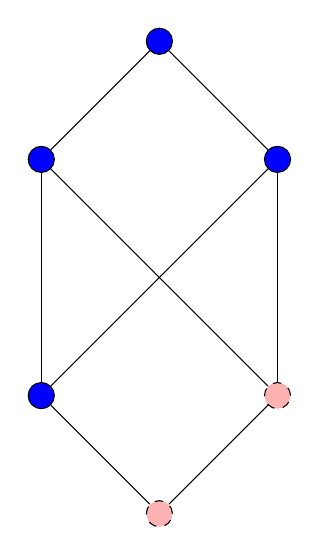
\begin{tikzpicture}[scale=1.5]

% Define nodes
\node (v1) at (0, 2) [circle, draw, fill=blue] {};
\node (v2) at (1, 1) [circle, draw, fill=blue] {};
\node (v3) at (1, -1) [circle, draw, fill=red!30, dashed] {};
\node (v4) at (0, -2) [circle, draw, fill=red!30, dashed] {};
\node (v5) at (-1, -1) [circle, draw, fill=blue] {};
\node (v6) at (-1, 1) [circle, draw, fill=blue] {};

% Draw edges
\draw (v1) -- (v2);
\draw (v2) -- (v3);
\draw (v3) -- (v4);
\draw (v4) -- (v5);
\draw (v5) -- (v6);
\draw (v6) -- (v1);

% Draw additional edges to form the diamond shape
\draw (v2) -- (v5);
\draw (v3) -- (v6);

\end{tikzpicture}
\end{document}